\section{制御則}
ロボカーがコースを走る際,直進コースではロボカーを安定させ可能な限り速く走らせ,カーブに差し掛かったときにはステアリングとステアリングのための減速が必要である.特に,カーブを曲がりきるためにはどれだけのステアリング角と速度にすべきか,またその目標角度に追従させるためにはどのような制御系を構成する必要があるのかを考えなければならない.ここでは,ステアリング角と速度の目標値生成および制御方法について説明する.
 
 
\subsection{RCサーボモータ}
ロボカーのステアリング角はRCサーボモータの角度により決められる.すなわち,RCサーボモータへの目標角度生成則について考える必要がある.
  
\subsubsection{構造}
RCサーボモータは内部でフィードバック制御が行われている.その構造は\refig{RC_construction}に示すとおりである\cite{RCservo}.目標角度に対応するPWM信号を入力すると内部で目標値に追従するように制御が行われる.

\subsubsection{目標値生成}
  本レースで走行させるロボカーは左右側面に設置された距離センサにより左右のコースの壁との距離をそれぞれ検出し,その距離の差によりステアリング角を変化させる.右側の壁との距離が左側の壁との距離より大きければステアリング角を時計回り方向に,小さければステアリング角を反時計回りに回転させる.ロボカーが直進コースを走行するときに比べ,カーブに差しかかったときとでは\refig{steering_compa}のように左右の壁との距離の差が大きくなる.すなわち,直進コースのように距離の差が小さくなるときにはRCサーボモータの角度を小さくしてロボカーが前方を向くようにし,大きくなるときにはRCサーボモータの角度を大きくすることでカーブに差しかかった場合に必要なステアリング角を実現することができる.また,直進コースではロボカーをコースの中央に位置させるようにステアリングを行わせることができる.
  
RCサーボモータでのPWM信号の周期は$16〜23\unit{msec}$であり,その周期中のパルス幅の大きさに比例してRCサーボモータの角度が決まる.周期$20\unit{msec}$のPWM信号のパルス幅を$0.9\unit{msec}$から$2.1\unit{msec}$まで変化させると,RCサーボモータの角度は\refig{RC_pulse}に示すように変化する.この特性よりPWM信号のパルス幅$W\unit{msec}$に対してRCサーボモータの角度$\theta=f(W)\unit{\deg}$とおく.距離センサの値の定義域は正規化により$[0.0,1.0]$となるので,左右の距離センサの値の差は$[-1.0,1.0]$の範囲で値をとる.この範囲で左右の距離の差の大きさに応じてステアリング角を大きくし,最大角度を超えないようにする必要がある.そのためシグモイド関数$\sigma_{a_{s}}(x_{s}) $を用いた次式で目標角度$\theta_{r} $を生成することにした.

\begin{equation}  
  \theta_{r} = f(W) =f(1.5-2\cdot0.6(\sigma_{a_{s}}(x_{s})-0.5))
\end{equation}

\begin{figure}[htb]

  \centering
    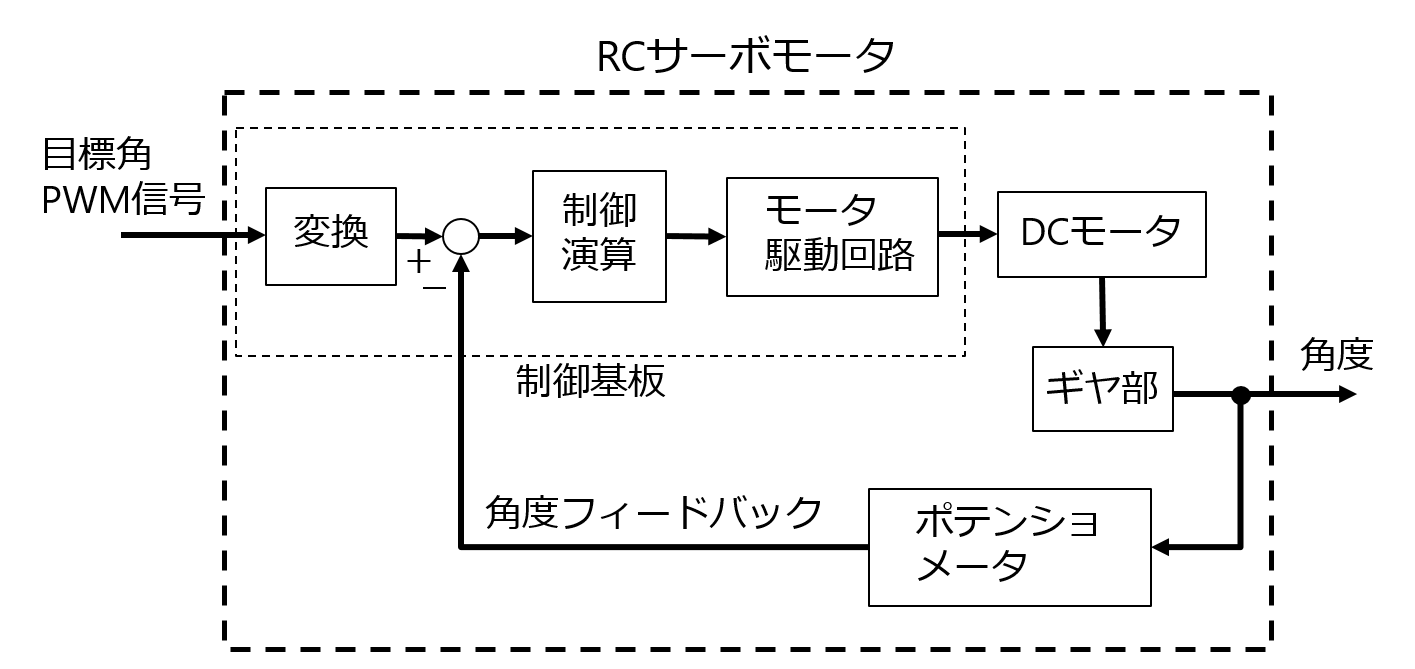
\includegraphics[width=0.7\hsize]{picture/eps/RC_construction.eps}
  \caption{RCサーボモータの制御系}
  \label{fig::RC_construction}
\end{figure} 

\begin{figure}[htb]

  \centering
    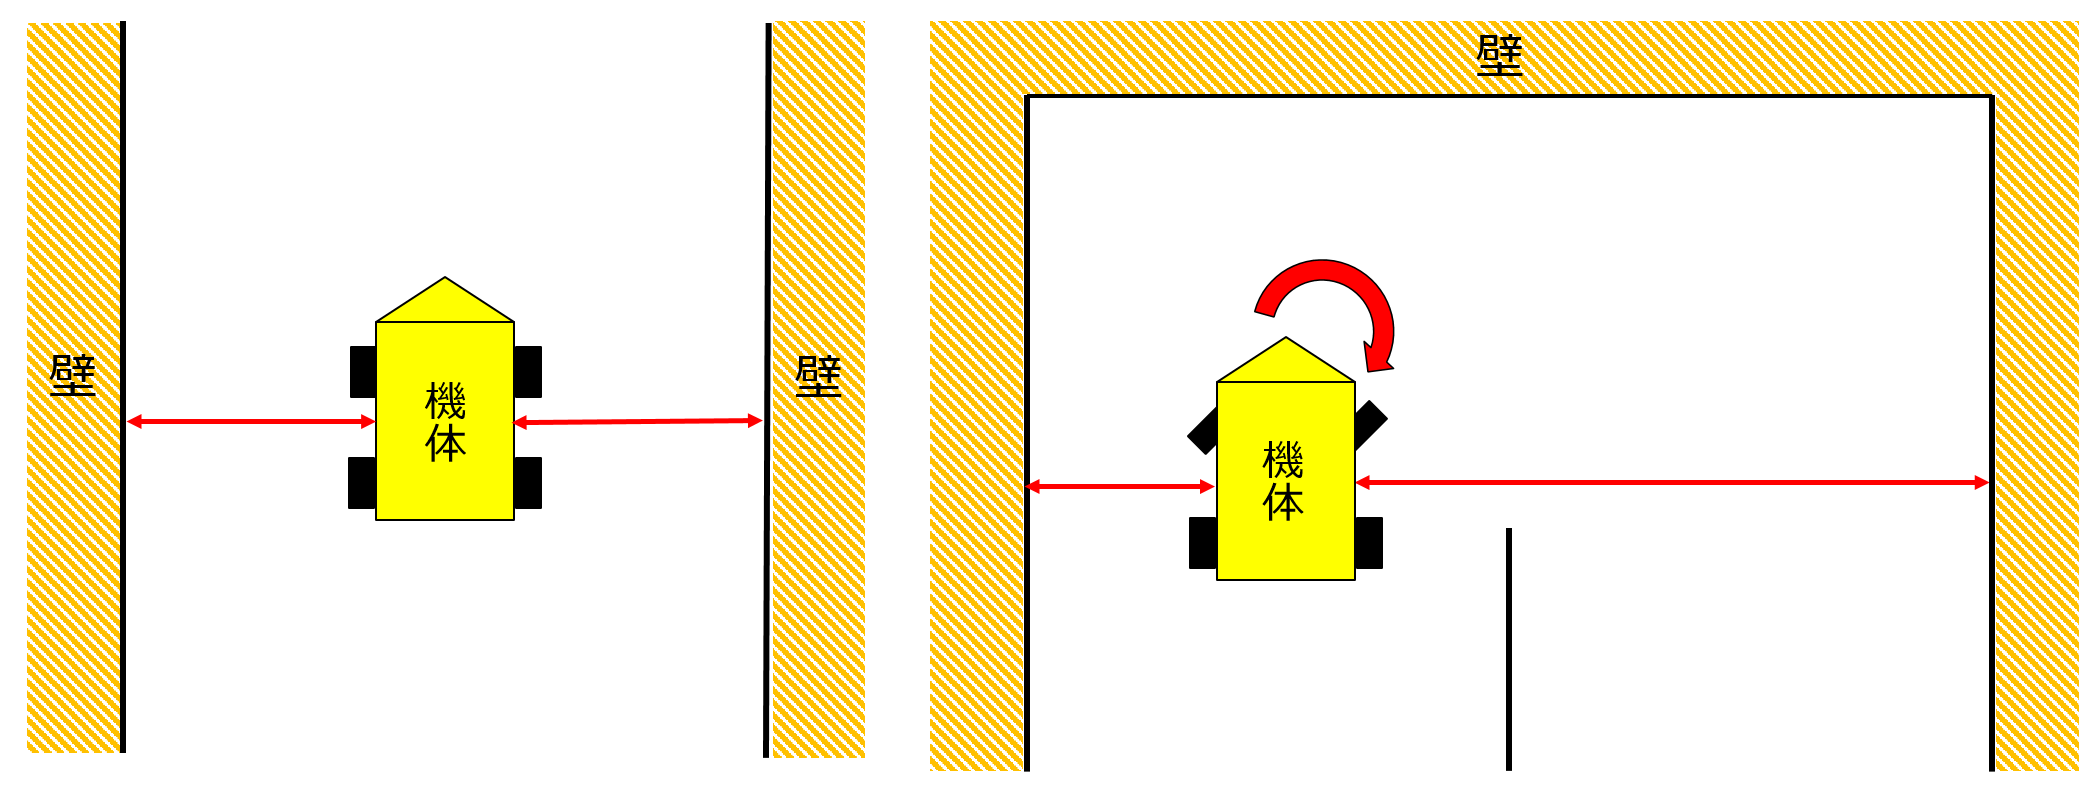
\includegraphics[width=0.8\hsize]{picture/eps/steering_compa.eps}
  \caption{直進コースとカーブとでの左右の壁との距離の差}
  \label{fig::steering_compa}
\end{figure}  

\begin{figure}[htb]

  \centering
    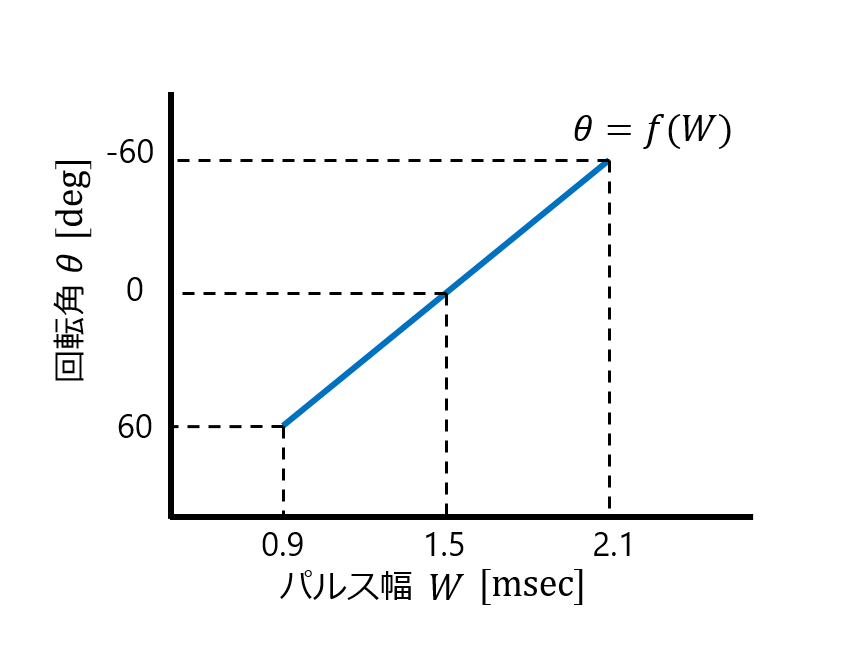
\includegraphics[width=0.5\hsize]{picture/eps/RC_pulse.eps}
  \caption{PWM信号のパルス幅とRCサーボモータの角度の関係}
  \label{fig::RC_pulse}
\end{figure} 
 
\newpage
ここで$ a_{s}$は正の定数であり,$ x_{s}$はロボカーの左右のセンサの値の差である.この式ではシグモイド関数$\sigma_{a_{s}}(x_{s}) $を$y$軸方向に$-0.5$だけ平行移動させ,その全体を$2$倍することで$(-\infty,\infty)$の定義域において$(-1.0,1.0)$の値域で変化するようにしている.さらに,$0.6$をかけることで値域を$(-0.6,0.6)$としている.式中の$1.5$は\refig{RC_pulse}でRCサーボモータの角度が$0\unit{deg}$となるときのPWM信号のパルス幅である.この式では左右のセンサの値の差によりPWM信号のパルス幅を変えることで目標角度$\theta_{r} $を決定している.\refig{RC_pulse}に示したように,左右のセンサの値の差がなければ$x_{s}=0\unit{\deg}$となりパルス幅は$1.5\unit{msec}$となって目標角度$\theta_{r}$は$0\unit{\deg}$となる.右のセンサの値が左のセンサの値より大きい場合を正とすれば,RCサーボモータの角度は右の壁との距離の方が大きくなると時計回りに大きくなり,左の壁との距離のほうが大きくなると反時計回りに大きくなる.定数$a_{s}$はシグモイド関数の変化の速さにかかわり,試走実験を通して適切な値とする必要がある.

\newpage
 \begin{figure}[htb]
  \centering
    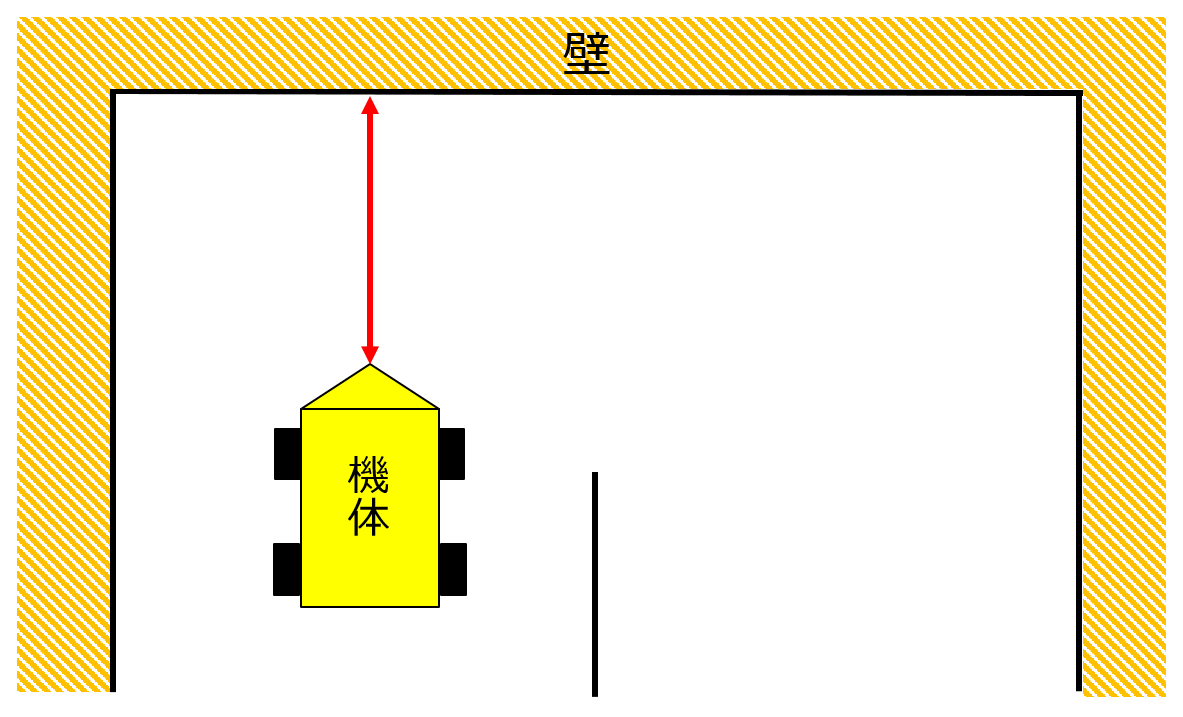
\includegraphics[width=0.6\hsize]{picture/eps/speed_wall.eps}
  \caption{前方の壁との距離に対する速度}
  \label{fig::speed_wall}
\end{figure}
\subsection{DCモータ}
ロボカーの速度はDCモータの角速度により決められる.すなわち,DCモータへの目標角速度生成と,その目標値に追従させるための制御方法を考える必要がある.

\begin{figure}[htb]
  \centering
    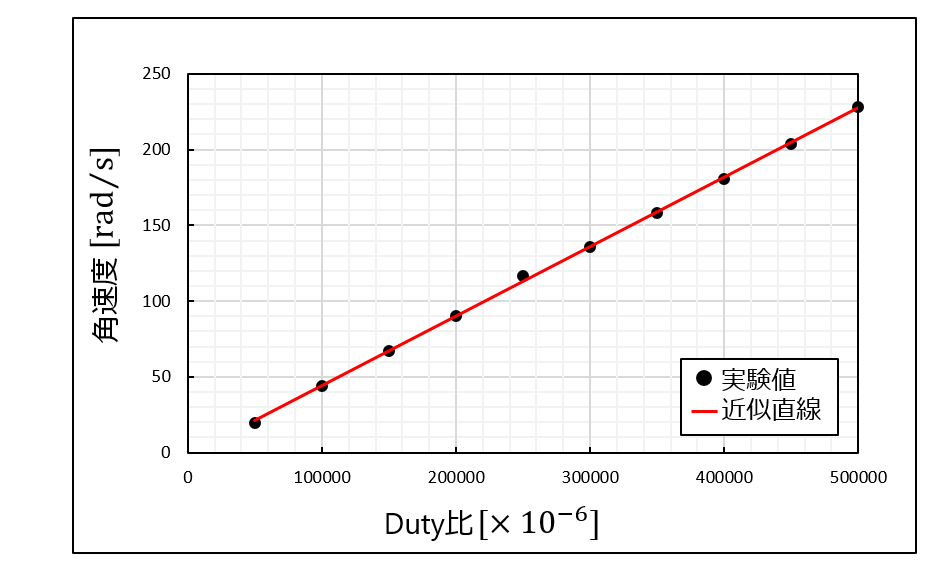
\includegraphics[width=0.7\hsize]{picture/eps/duty_angvel_graph.eps}
  \caption{PWM信号のDuty比とDCモータの角速度との関係}
  \label{fig::duty_angvel_graph}
\end{figure}

\subsubsection{PWM信号とDCモータの角速度}
以下のようにして,PWM信号とDCモータの角速度との関係式を導いた.
\begin{enumerate}
\item DCモータにDuty比$0.05$のPWM信号を与え,定常となったときのDCモータの角速度の値を記録した.この値は定常時でのDCモータの角速度の値を平均化して求めた.なお,与えるDuty比はプログラムの関係上,実際のDuty比を$10^{6}$倍して与えている.
\item DCモータに与えるPWM信号のDuty比を$0.05$刻みで$0.5$まで増加させ,各Duty比の場合ごとに(1)と同様の操作を行った.
\item 各Duty比のPWM信号に対するDCモータの角速度は\refig{duty_angvel_graph}に示すようになった.これに対し近似直線を引けば,PWM信号のDuty比を$d[\times 10^{-6}]$,DCモータの角速度を$\omega\unit{rad/s}$とおいたときその式は
\begin{equation}
\omega=0.0005\times d-1.861 \label{eq::omega_pulse}
\end{equation}
と表せた.この式より,DCモータの角速度からPWM信号のDuty比を求める式は
\begin{equation}
d=2178\times\omega-4176 \label{eq::pulse_omega}
\end{equation}
と表せた.
\end{enumerate} 
\refeq{omega_pulse}よりPWM信号のDuty比が最大となったときのDCモータの角速度を求めることができ,\refeq{pulse_omega}より任意のDCモータの角速度を与えるのに必要なPWM信号のDuty比を求めることができる.
\subsubsection{目標値生成}
カーブを曲がりきるためには,ステアリングに余裕をもたせるための減速が必要である.本レースで走行させるロボカーは,正面に設置された距離センサにより前方の壁との距離を検出し,その距離に応じて速度を変化させる.\refig{speed_wall}のようにカーブに差しかかれば正面のコースの壁との距離は小さくなる.すなわち,正面のコースの壁との距離が小さくなるほどDCモータの角速度を小さくすることでカーブでの減速を実現することができる.壁との距離に比例して目標角速度を生成すると,壁との距離が大きくなるほどDCモータの角速度が大きくなりモータの最大角速度まで大きくなってしまう.DCモータの角速度が最大の状態でロボカーを走らせると消費電力が大きくなり電源の消耗が速くなったり,ロボカーがモータの回転に耐えられないなどの問題が生じる.この問題を解消するためには最大角速度をある値までに抑え,前方の壁との距離が一定以上大きくなるとそれ以上角速度が大きくならないようにする必要がある.なおかつ,壁との距離が小さくなれば速度を落としたいので,DCモータの角速度の目標値生成にはRCサーボモータと同様にシグモイド関数$\sigma_{a_{d}}(x_{d})$を用いることにした.指定最大角速度を$\omega_{max}\unit{rad/s} $とすれば,DCモータへの目標角速度$\omega_{r}\unit{rad/s}$は次式で生成される.
\begin{equation}
 \omega_{r}=\omega_{max}\sigma_{a_{d}}(x_{d}-b)\label{eq::omega_r}
\end{equation}
ここで,$a_{d}$,$b$は正の定数であり,$x_{d}$は前方の距離センサの値である.定数$a_{d}$はシグモイド関数の変化の速さに関わる.距離センサの値は正規化されているので$x_{d}$の定義域は$[0.0,1.0]$となる.シグモイド関数$\sigma_{a}(x)$は前方の壁との距離に対し増減し,値域は$(0.0,1.0)$である.センサの値が$0.0$のときにはシグモイド関数の値は$0.5$となる.これでは前方の壁との距離がどれだけ小さくなっても指定最大角速度の半分までしか減速できないため,指定最大角速度が大きくなるほど最低角速度が大きくなりステアリングのための減速が十分に行えなくなってしまう.正の定数$b$だけシグモイド関数を$x$軸方向に平行移動させることで,最低角速度を指定最大角速度の半分より小さくできる.以上より\refeq{omega_r}を与えることで,壁との距離がどれだけ離れても目標角速度$\omega_{r}\unit{rad/s}$は指定最大角速度$\omega_{max}\unit{rad/s}$に抑えられ電力消費を抑えることができ,前方の壁との距離が小さくなるカーブにおいてステアリングのための減速を行うことができる.正の定数$a_{d}$と$b$の値は試走実験を通して適切な値に決める必要がある.

\subsubsection{モデリング}
DCモータの代表的な等価回路を\refig{dcm_circit}に示す.\cite{dcmmodeling}ただし,モータへの入力電圧を$v\unit{V}$,電機子電流を$i_{a}\unit{A}$,電機子抵抗を$R_{a}\unit{\Omega}$,自己インダクタンスを$L_{a}\unit{H}$,誘起電圧定数を$K_{E}\unit{Vs/rad}$,電機子の回転角速度を$\omega_{m}\unit{rad/s}$,電機子に発生するトルクを$T\unit{Nm}$,負荷トルクを$T_L\unit{Nm}$,回転子と負荷の合成慣性モーメントを$J\unit{kg\cdot m^2}$とする.以下ではこの等価回路に沿ってDCモータの定式化を行う.

\refig{dcm_circit}より,DCモータの支配方程式は次のように書ける.
\begin{align}
v &= K_{E}\omega_{m} + R_{a}i_{a} + L_{a}\frac{di_{a}}{dt} \label{eq::dcm_v} \\
T &= J\frac{d\omega_{m}}{dt} + T_{L} \label{eq::dcm_t}
\end{align}

\refeq{dcm_v},\refeq{dcm_t}より\refig{dcm_block}のブロック線図を得る.
ここで,図中の$J$はモータ回転子の慣性モーメント$J_{M}$と負荷の慣性モーメント$J_{L}$の和を表し,
$K_{T}\unit{Nm/A}$はDCモータのトルク定数である.
\refig{dcm_block}より負荷を含まないDCモータ単体の伝達関数$G_{M}(s)$を求めると以下のようになる.
\begin{align}
G_{M}(s) &= \frac{\Omega_{m}(s)}{V(s)} = 
\frac{\cfrac{K_{T}}{(R_{a} + L_{a}s)J_{M}s}}{1 + \cfrac{K_{T}K_{E}}{(R_{a} + L_{a}s)J_{M}s}} \nonumber \\
 &= \frac{\cfrac{1}{K_{E}}}{1 + \cfrac{R_{a}J_{M}}{K_{T}K_{E}}s + \cfrac{L_{a}J_{M}}{K_{T}K_{E}}s^2} \label{eq::dcm_tf}
\end{align}

ただし,$\Omega_{m}(s) = \mathcal{L}\{\omega_{m}(t)\},V(s) = \mathcal{L}\{v(t)\}$である.

\refeq{dcm_tf}より,電流の増加を遅らせるインダクタンスと回転角速度の上昇を遅らせる慣性モーメントという2つのエネルギ蓄積素子が二次のダイナミクスをつくっている事がわかる.

\begin{figure}[htb]
  \centering
    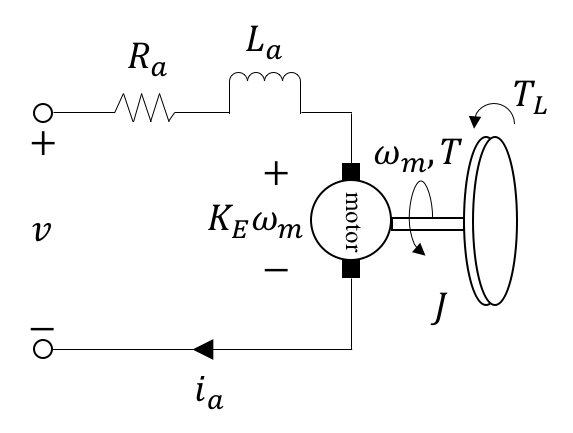
\includegraphics[width=0.5\hsize]{picture/eps/dcm_circit.eps}
    \caption{DCモータの等価回路}
    \label{fig::dcm_circit}
\end{figure}

\begin{figure}[htb]
  \centering
    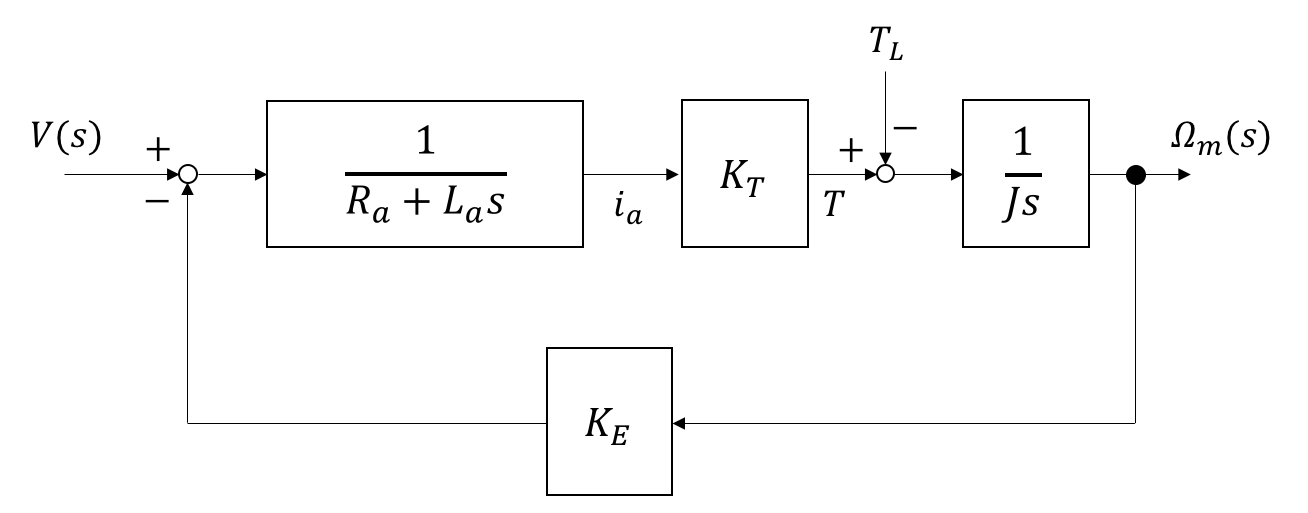
\includegraphics[width=1.0\hsize]{picture/eps/dcm_block_diagram.eps}
    \caption{DCモータのブロック線図}
    \label{fig::dcm_block}
\end{figure}


\subsubsection{制御系}
DCモータの入力電圧から出力角速度への伝達関数を$G(s)$をとおく.DCモータの入力電圧から出力角速度への伝達関数は\refeq{dcm_tf}に示すように二次遅れ系となる.モデルを簡単にするためステップ応答法を用いて次式のように一次遅れ+むだ時間系に近似することにした.  
\begin{equation}
 G(s)=\frac{Ke^{-Ls}}{1+Ts}
\end{equation} 
$K$はゲイン,$T$は時定数,$L$はむだ時間である.ステップ応答法を用いて,以下のようにDCモータの入力電圧から出力角速度への伝達関数を求め,同定を行った.

\begin{enumerate}
\item 電圧$7.2\unit{V}$,Duty比$0.1$のPWM信号を加え,DCモータの角速度が定常になるまでの応答を記録した.この応答を\refig{dcmotor_response}に示す.このとき入力電圧は電圧とDuty比の積である$0.72\unit{V}$に相当し,定常での角速度は$30.74\unit{rad/s}$であるのでゲイン$K$は
\begin{equation}
 K=\frac{30.74}{0.72}=42.69
\end{equation}
となる.
\item (1)で得られた応答について,\refig{step_doutei}に示すように応答の変曲点で接線を引くことで時定数$T$とむだ時間$L$を求めた.$T$,$L$は以下の値となった.
\begin{align}
 T&=0.031 \\
 L&=0.006
\end{align}
\item(1),(2)よりDCモータの入力電圧から角速度への伝達関数は次式のようになった.
\begin{equation}
 G(s)=\frac{42.69e^{-0.006s}}{1+0.031s}
\end{equation} 
この伝達関数より同定した曲線を\refig{dcmotor_doutei}に示す.
\end{enumerate}

\begin{figure}[htb]
  \centering
    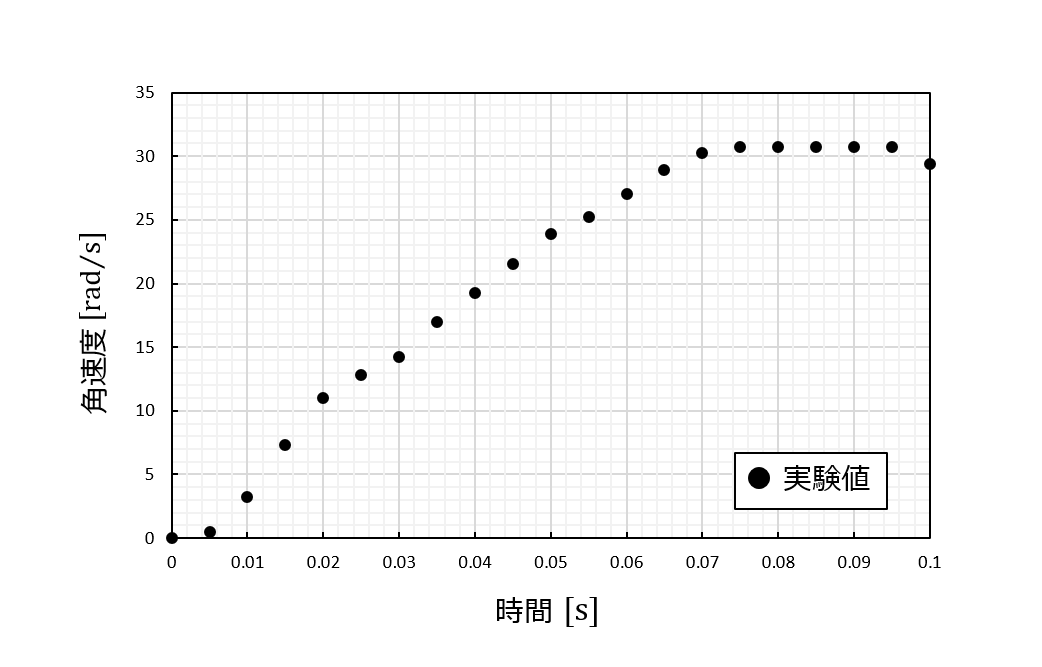
\includegraphics[width=0.7\hsize]{picture/eps/dcmotor_response.eps}
  \caption{DCモータのステップ応答}
  \label{fig::dcmotor_response}
  
\end{figure}

\begin{figure}[htb]
  \centering
    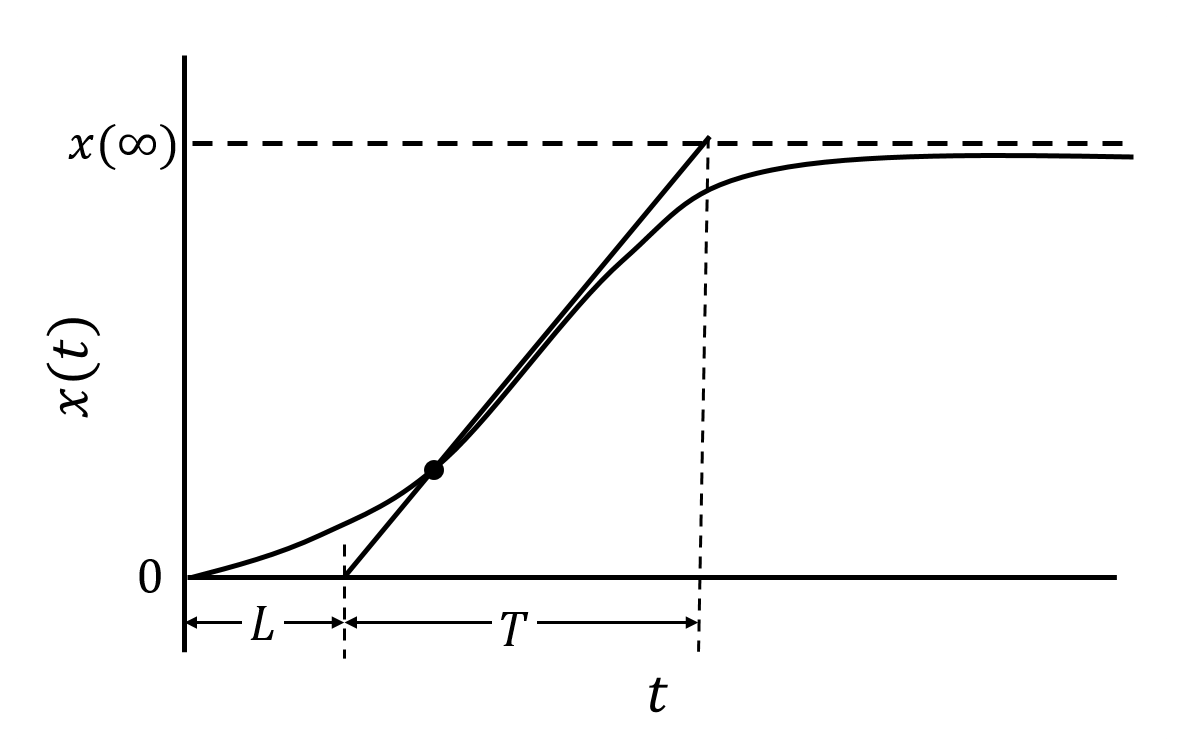
\includegraphics[width=0.7\hsize]{picture/eps/step_doutei.eps}
  \caption{ステップ応答から$T$と$L$を求める方法}
  \label{fig::step_doutei}
  
\end{figure}

\begin{figure}[htb]
  \centering
    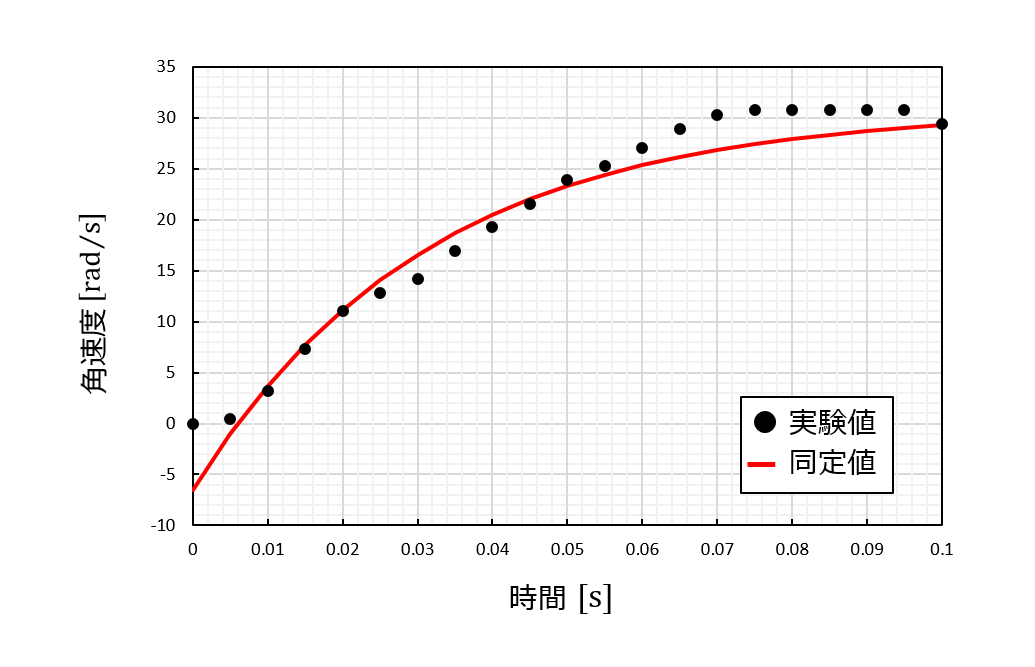
\includegraphics[width=0.7\hsize]{picture/eps/dcmotor_doutei.eps}
  \caption{DCモータの同定結果}
  \label{fig::dcmotor_doutei}
  
\end{figure}

  
DCモータの制御系は,\refig{pi_control}に示すようにPI制御器を用いた閉ループ系で構成する.PI制御器を用いるのは,DCモータの角速度を目標角速度へ速やかに到達させるためである.PI制御器中の$K_{p}$,$K_{i}$は順に比例ゲイン,積分ゲインである.これらのパラメータの値をボード線図を用いて以下に決定した.
まず,伝達関数$G(s)$とPI制御器のそれぞれについてボード線図での折れ点周波数を求めた.$G(s)$の折れ点周波数を$\omega_{1}$とおくと,その値は  
\begin{equation}
 \omega_{1}=\frac{1}{T}=32.25\unit{rad/s}
\end{equation}
となった.一方,PI制御器の折れ点周波数はPI制御器の式を
\begin{equation}
 K_{p}+\frac{K_{i}}{s}=K_{p}(1+\frac{\omega_{PI}}{s})
\end{equation}
と変形したときの$\omega_{PI}$である.ただし,
\begin{equation}
 \omega_{PI}=\frac{K_{i}}{K_{p}}\label{eq::omega_PI}
\end{equation}
である.

次に,伝達関数$G(s)$とPI制御器のそれぞれについてゲインと位相を求めた.
伝達関数$G(s)$,PI制御器のゲインをそれぞれ$g_{s},g_{PI}$,位相をそれぞれ$\phi_{s},\phi_{PI}$とおく.このとき$s=j\omega$とおけば,
\begin{align}
 g_{s}&=20\log_{10}{|G(j\omega)|}=20\log_{10}{\frac{K}{\sqrt{1+(\omega T)^{2}}}} \\
 \phi_{s}&=-\tan^{-1}{\omega T}-\omega L \\
 g_{PI}&=20\log_{10}{|K_{p}+\frac{K_{i}}{j\omega}|}=20\log_{10}{\sqrt{K_{p}^{2}+(\frac{K_{i}}{\omega})^{2}}} \\
 \phi_{PI}&=-\tan^{-1}{\frac{K_{i}}{K_{p}\omega}}
\end{align}
と各ゲイン,位相の式が求められた.ここで,PI制御器+伝達関数$G(s)$の開ループ伝達関数のゲイン,位相をそれぞれ$g_{c},\phi_{c}$とおく.これらの式は伝達関数$G(s)$とPI制御器のゲイン,位相をそれぞれ足し合わせて表せるので$g_{c},\phi_{c}$の式は
\begin{align}
 g_{c}&=g_{s}+g_{PI}\\
 \phi_{c}&=\phi_{s}+\phi_{PI}
\end{align}
となった.これらの式よりPI制御器+伝達関数$G(s)$のボード線図を描くことができる.

\begin{figure}[htb]
  \centering
    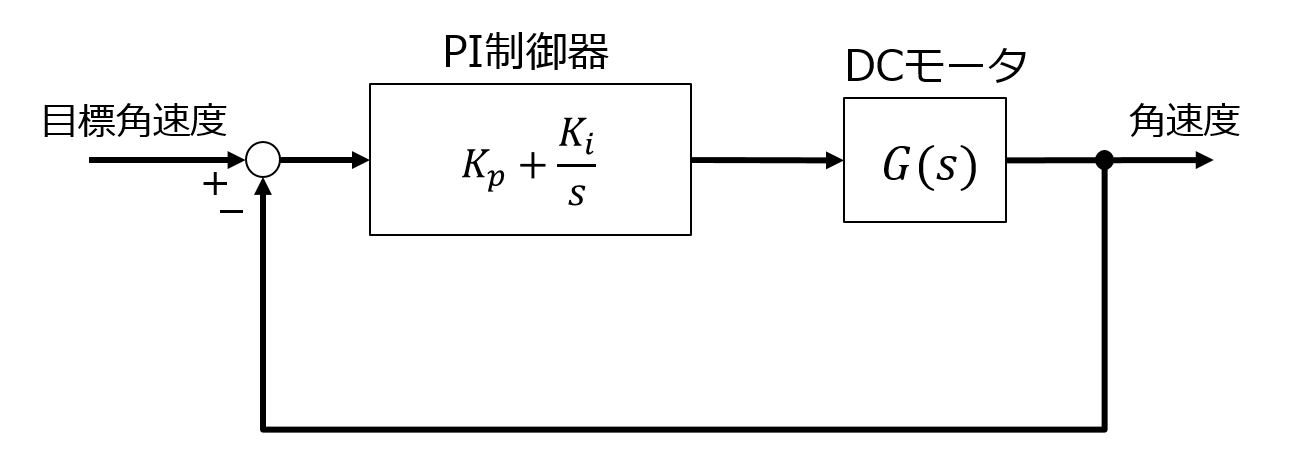
\includegraphics[width=0.7\hsize]{picture/eps/pi_control.eps}
  \caption{DCモータの制御系}
  \label{fig::pi_control}
  
\end{figure}

\begin{figure}[htb]
  \centering
    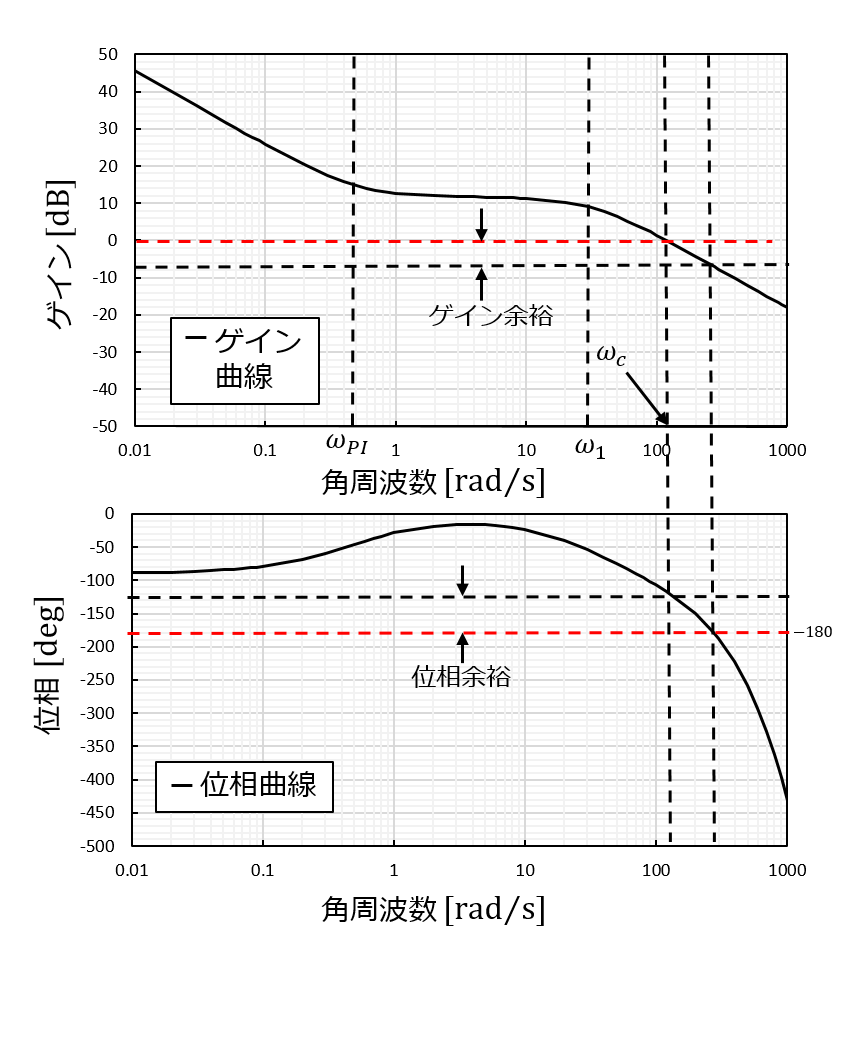
\includegraphics[width=0.6\hsize]{picture/eps/pi_board.eps}
  \caption{PI制御器+伝達関数$G(s)$のボード線図}
  \label{fig::pi_board}
  
\end{figure}

\newpage

DCモータの角速度を目標値に追従させる制御を行うために以下のようにしてPI制御器+伝達関数$G(s)$のボード線図を描いた.

\begin{enumerate}
\item PI制御器+伝達関数$G(s)$のボード線図について,ゲイン交差周波数(ゲインが$0\unit{dB}$となるときの角周波数)を$\omega_{c}$とおく.このとき,伝達関数$G(s)$の折れ点周波数$\omega_{1}$に対して,PI制御器の折れ点周波数$\omega_{PI}$は$\omega_{1}$より数倍程度小さく,$\omega_{c}$は数倍程度大きくなるように設定するようにした.一般にサーボ系ではゲイン余裕を$12〜20\unit{dB}$,位相余裕を$40〜60\unit{deg}$とするのがよいとされるので,これらの値を目安にして$\omega_{c}$,$\omega_{PI}$の値を変えることでゲイン余裕,位相余裕の値を調整した.また,$\omega_{c}$を大きくすれば速応性が大きくなるほど速くなるが,負荷の共振現象が存在する場合に負荷の振動を助長してしまうため大きくし過ぎないように設定することにした.これらの条件より
\begin{align}
 \omega_{PI}&=0.5\unit{rad/s}\label{eq::omega_PI_value}\\
 \omega_{c}&=120\unit{rad/s}\label{eq::omega_c_value}
\end{align}
とした.
\item ゲイン交差周波数$\omega_{c}$付近ではゲインの傾きが$-20\unit{dB/sec}$となるのが望ましく,角周波数がゲイン交差周波数$\omega_{c}$のときには次の等式が成り立つ.
\begin{equation}
|G(j\omega_{c})\cdot(K_{p}+\frac{K_{i}}{j\omega_{c}})|=1\label{eq::omega_c_1}
\end{equation}
\item \refeq{omega_PI_value},\refeq{omega_c_value}の値を用いて,\refeq{omega_PI},\refeq{omega_c_1}を連立して解くと,比例ゲイン$K_{p}$,積分ゲイン$K_{i}$は以下のように求まった.
\begin{align}
K_{p}&=0.090\label{eq::K_p_value}\\
K_{i}&=0.045\label{eq::K_i_value}
\end{align}
PI制御器のゲインをこのように設定したとき,PI制御器+伝達関数$G(s)$のボード線図は\refig{pi_board}に示すとおりである.このときのゲイン余裕,位相余裕は以下のとおりであった.
\begin{align}
ゲイン余裕:7.14\unit{dB}\\
位相余裕:63.6\unit{deg}
\end{align}
\refeq{K_p_value},\refeq{K_i_value}の値を用いたPI制御器では,一般にサーボ系で良いとされるゲイン余裕,位相余裕を得ることはできなかった.ゲイン交差周波数$\omega_{c}$付近でゲインの傾きを$-20\unit{dB/sec}$にでき,$\omega_{PI}$,$\omega_{c}$,$\omega_{1}$が互いに干渉しないようにボード線図を描けたのでこのPI制御器を用いて\refig{pi_control}のような閉ループ制御系を構成した.
\end{enumerate}
構成した閉ループ制御系に対して,DCモータの角速度追従実験を行った.目標角速度は$150\unit{rad/s}$とした.このときの応答を\refig{pi_response}に示す.応答は目標角速度$150\unit{rad/s}$に$0.3\unit{s}$で到達して定常となった.これより,目標角速度への追従が実現できたといえる.

\begin{figure}[htb]
  \centering
    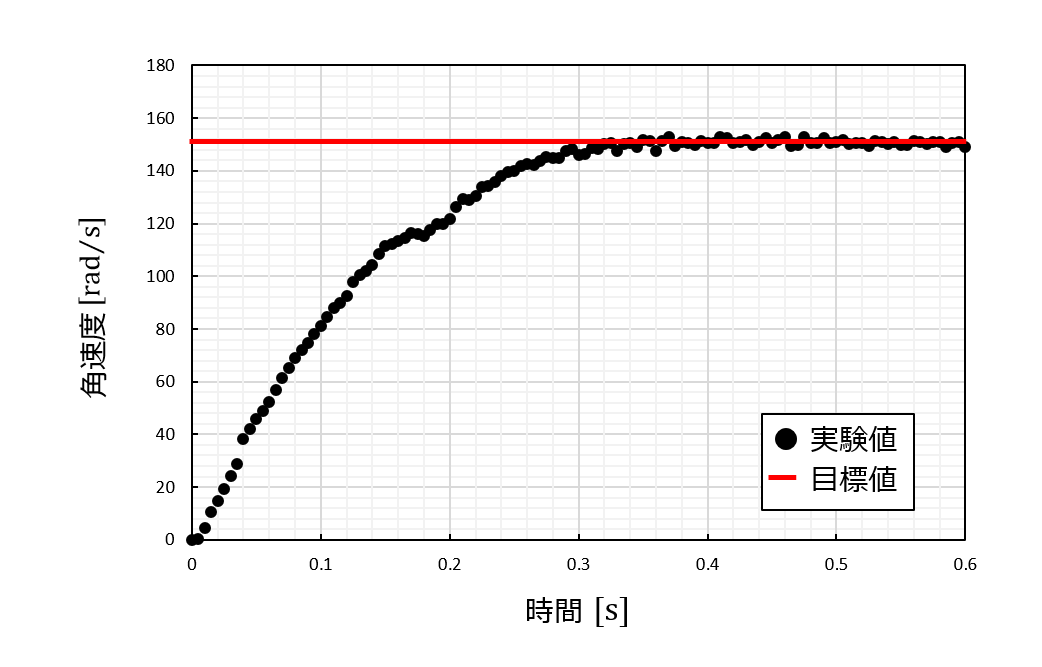
\includegraphics[width=0.7\hsize]{picture/eps/pi_response.eps}
  \caption{閉ループ制御系の応答}
  \label{fig::pi_response}
  
\end{figure}
